
% submission details
\newcommand{\deadlineOneTime}{noon}
\newcommand{\deadlineOneDate}{6 February 2020}
\newcommand{\submissionOneURL}{https://tabula.warwick.ac.uk/coursework/submission/0d913a74-f440-4f72-afd4-d84cb6ada99a}

%\renewcommand{\instructions}{Due at \emph{\deadlineTime} on \emph{\deadlineDate}.}


\cleardoublepage
\chapter{Coursework I}

\section{The Large Arithmetic Collider}

The goal of this coursework is to implement a Haskell program which can solve a challenging combinatorial game, which we refer to as the \emph{large arithmetic collider}. The game is based on a grid containing mathematical operations. To explain how it works, let us start with a simple example. Consider the following 4x1 sized grid containing the operations $+31$, $-26$, $-14$, $-1$ from left to right:
\begin{center}
	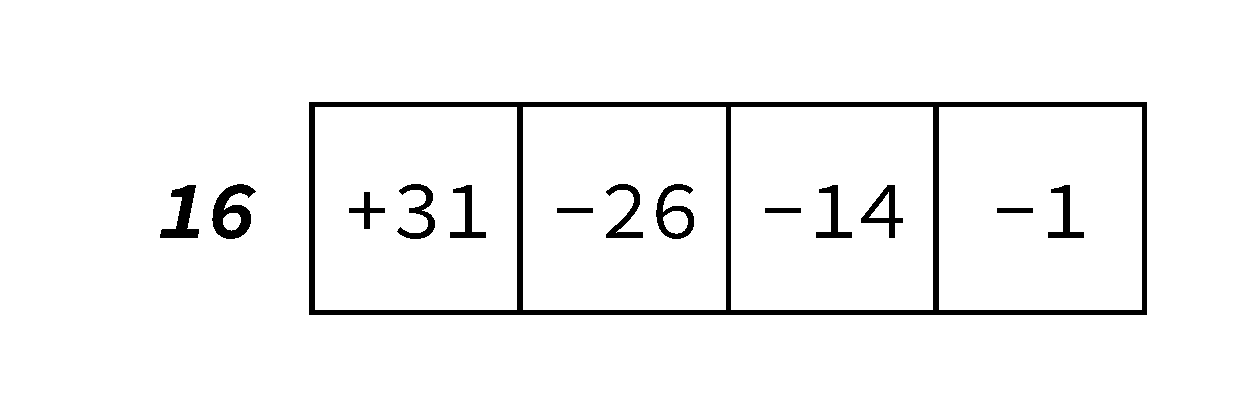
\includegraphics[scale=0.4,trim=0 30 0 30]{cswk/lac1.pdf}
\end{center}
You will also note that this row is annotated with the number $16$. The goal is to determine which of the operations contained in the cells result in that number when applied from left to right, starting with $0$. The solution for this simple example is shown below, where the cells containing operations that can be used to obtain the target number are shaded in grey:
\begin{center}
	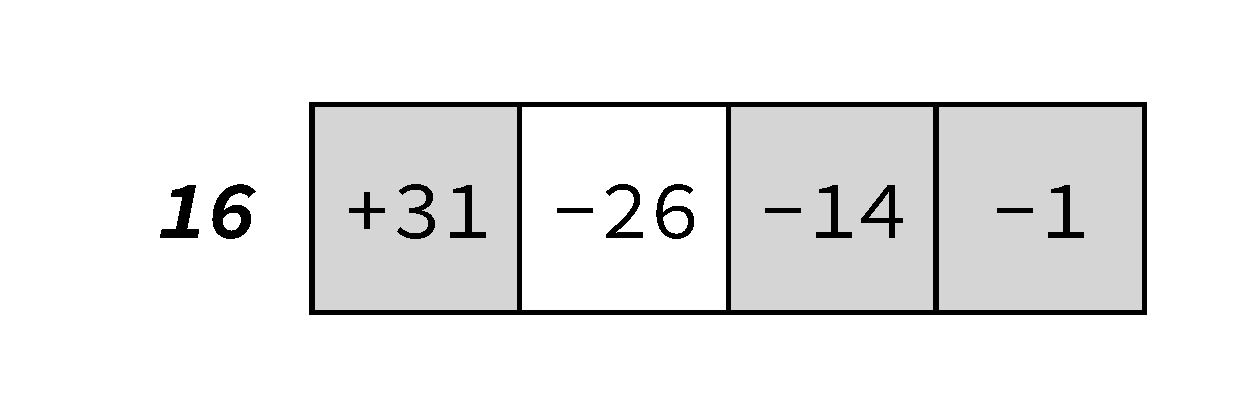
\includegraphics[scale=0.4,trim=0 30 0 30]{cswk/lac1s.pdf}
\end{center}
As we can easily see here, this is a solution because $0+31-14-1=16$. Since there are 4 cells in this example and each cell can either be used or not, there are $2^4=16$ possible configurations to explore here when searching for a solution. Although there is only one solution for this example, in general each grid may have more than one solution or, indeed, no solution. 

You may notice that we are talking about a ``grid'', but have only shown a single row to illustrate the basic game mechanics so far. A more realistic grid is shown below:
\begin{center}
	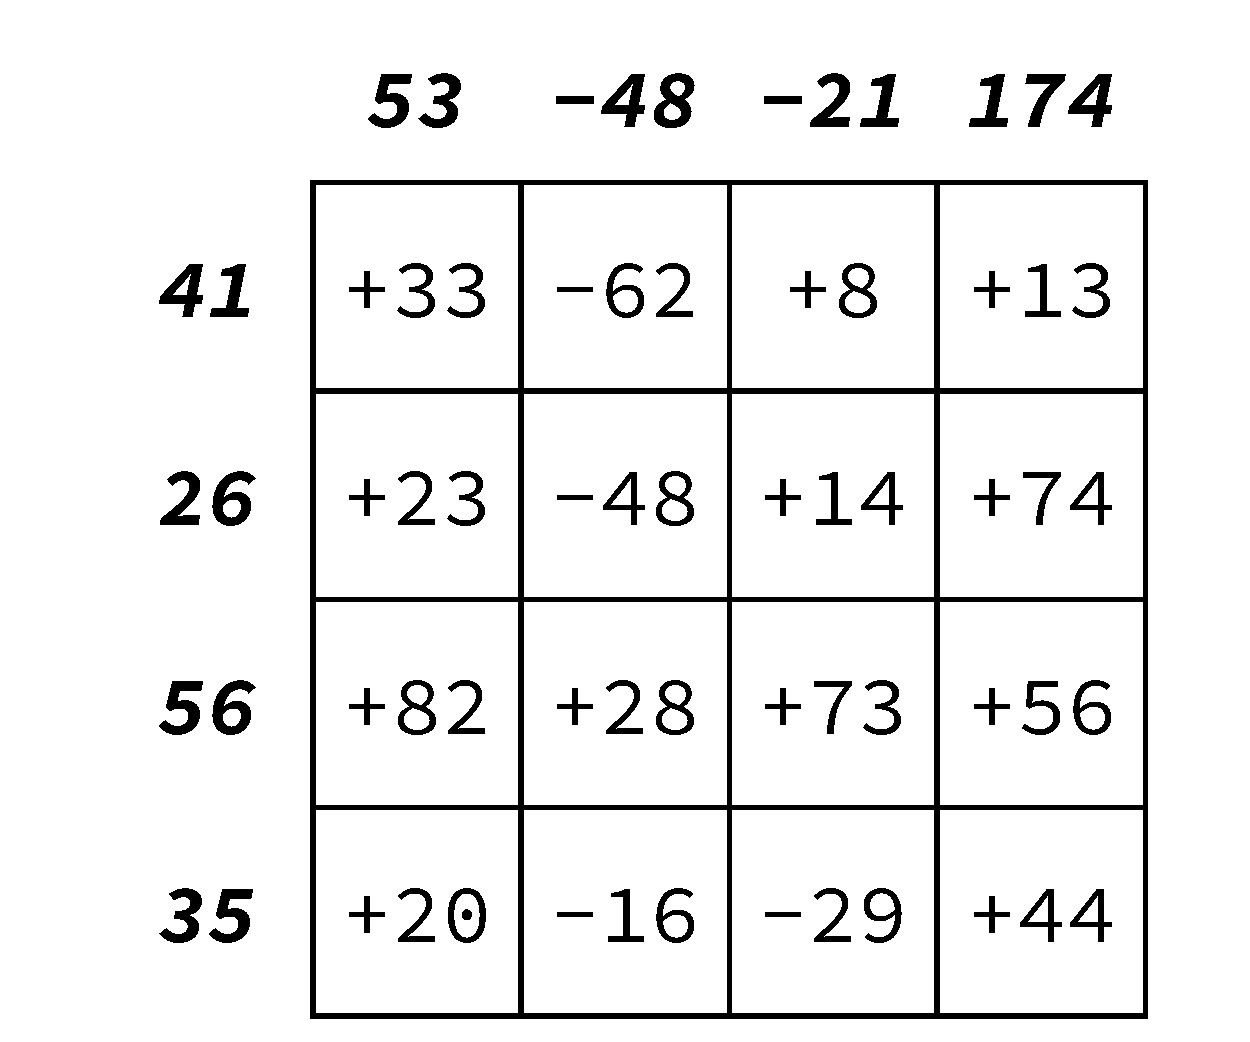
\includegraphics[scale=0.4,trim=0 30 0 30]{cswk/lac2.pdf}
\end{center}
As we can see, every row and every column is annotated with a target number. We must find which operations to use so that each row results in its target number as described in the previous example, but so that each column also results in its target number. The rules for columns are the same as for rows: we start with 0 and apply each active operation from top to bottom. The solution for this grid is shown below:
\begin{center}
	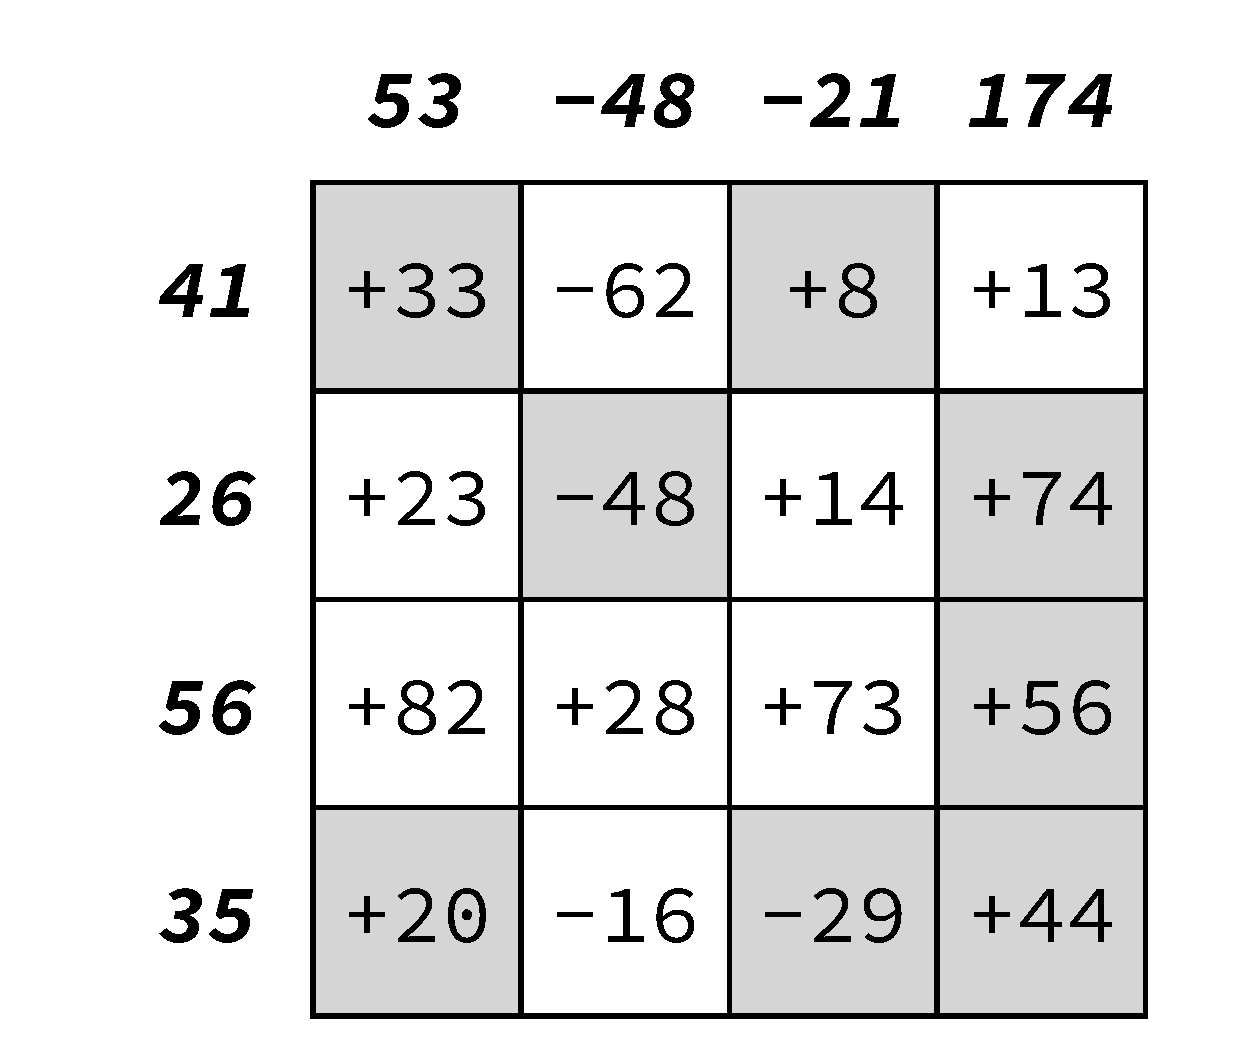
\includegraphics[scale=0.4,trim=0 30 0 30]{cswk/lac2c.pdf}
\end{center} 
Finding a solution for this grid is significantly more difficult. There are $4 \times 4 = 16$ cells and the number of possible configurations to explore is therefore $2^{16} = 65535$. Fortunately, this is still fairly simple for a computer to solve. At this point, you are encouraged to skip ahead to \Cref{sec:cswk1-getting-started} and implement the code required to solve grids using these mechanics.

\subsection{Advanced gameplay}

To further increase the difficulty of the game, there is one more game mechanic: the grids we have encountered so far can all be solved as they are, but we can also consider grids where rows or columns must be \emph{rotated} first. For example, consider the following grid:
\begin{center}
	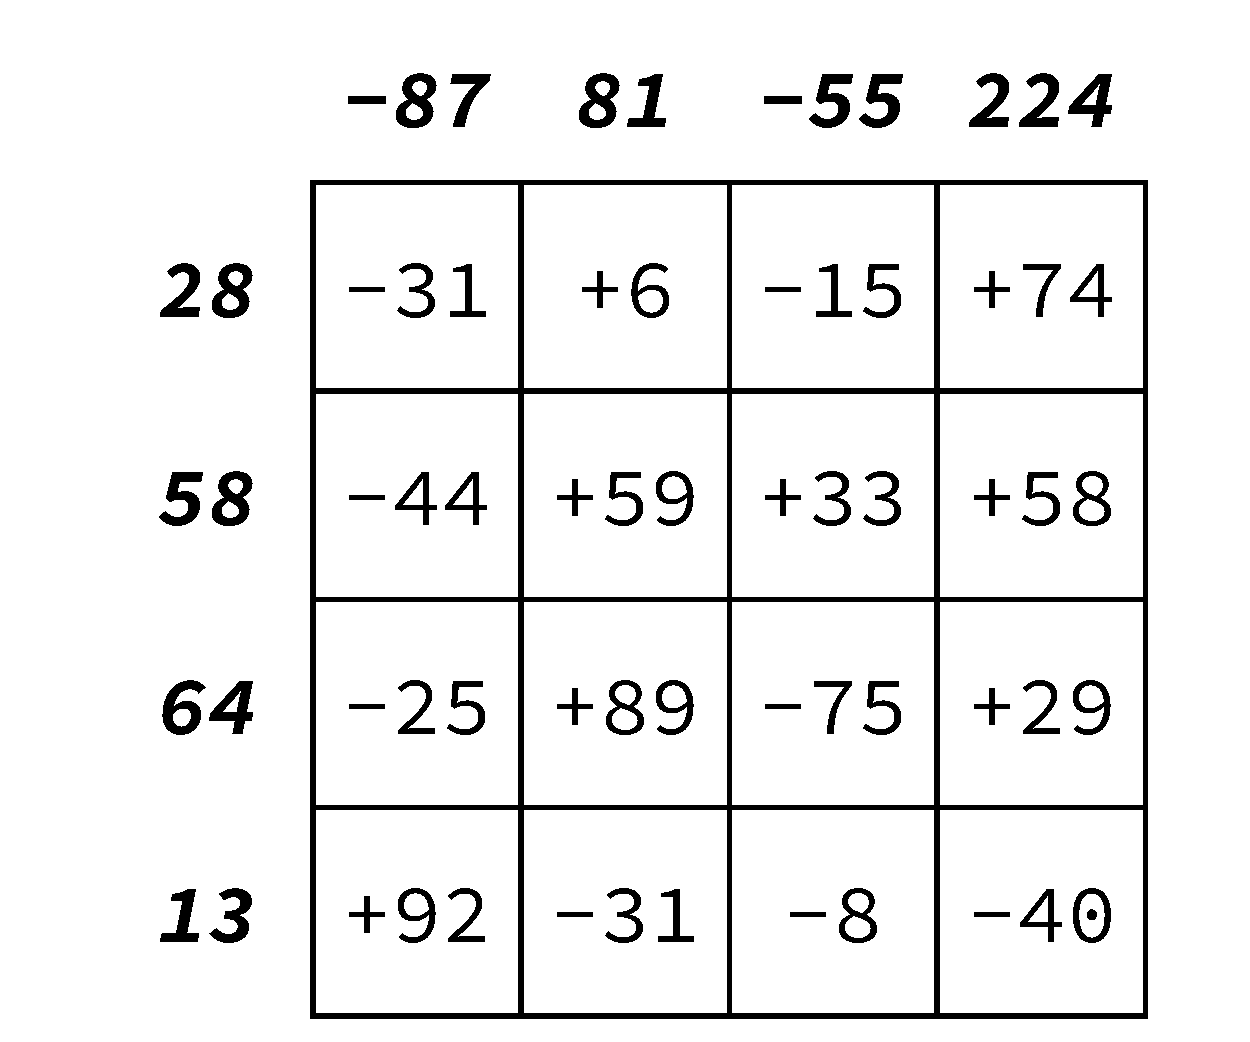
\includegraphics[scale=0.4,trim=0 30 0 30]{cswk/lac3.pdf}
\end{center}
This grid has no solutions as it is. However, we can find solutions if we change the layout of the cells by rotating some of the rows or columns. The rules for this are as follows: we can rotate one row or column at a time. We refer to this as one \emph{move}. Grids which can be solved without any rotations are solved in 0 moves. If a grid cannot be solved in 0 moves, then our goal is to try and solve it in as few moves as possible. For the example shown above, we can solve it in one move by rotating the last row of the grid:
\begin{center}
	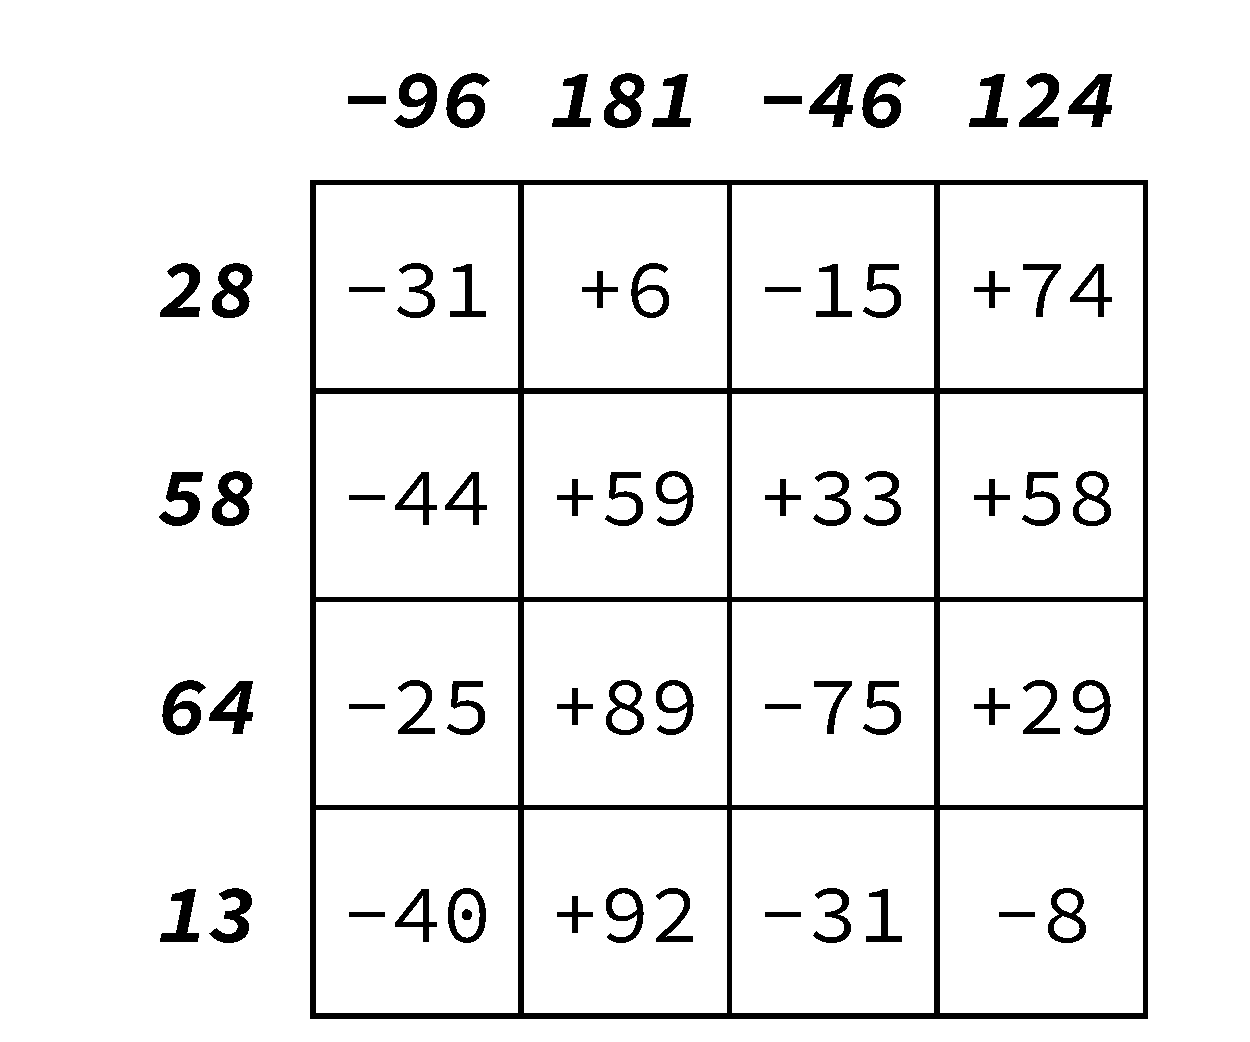
\includegraphics[scale=0.4,trim=0 30 0 30]{cswk/lac3r.pdf}
\end{center}
Rotations are always performed from left to right or top to bottom. Therefore, there are always $\mathit{rows}+\mathit{columns}$-many possible rotations at any given step. With the last rotated as shown, there is now a solution for the resulting grid:
\begin{center}
	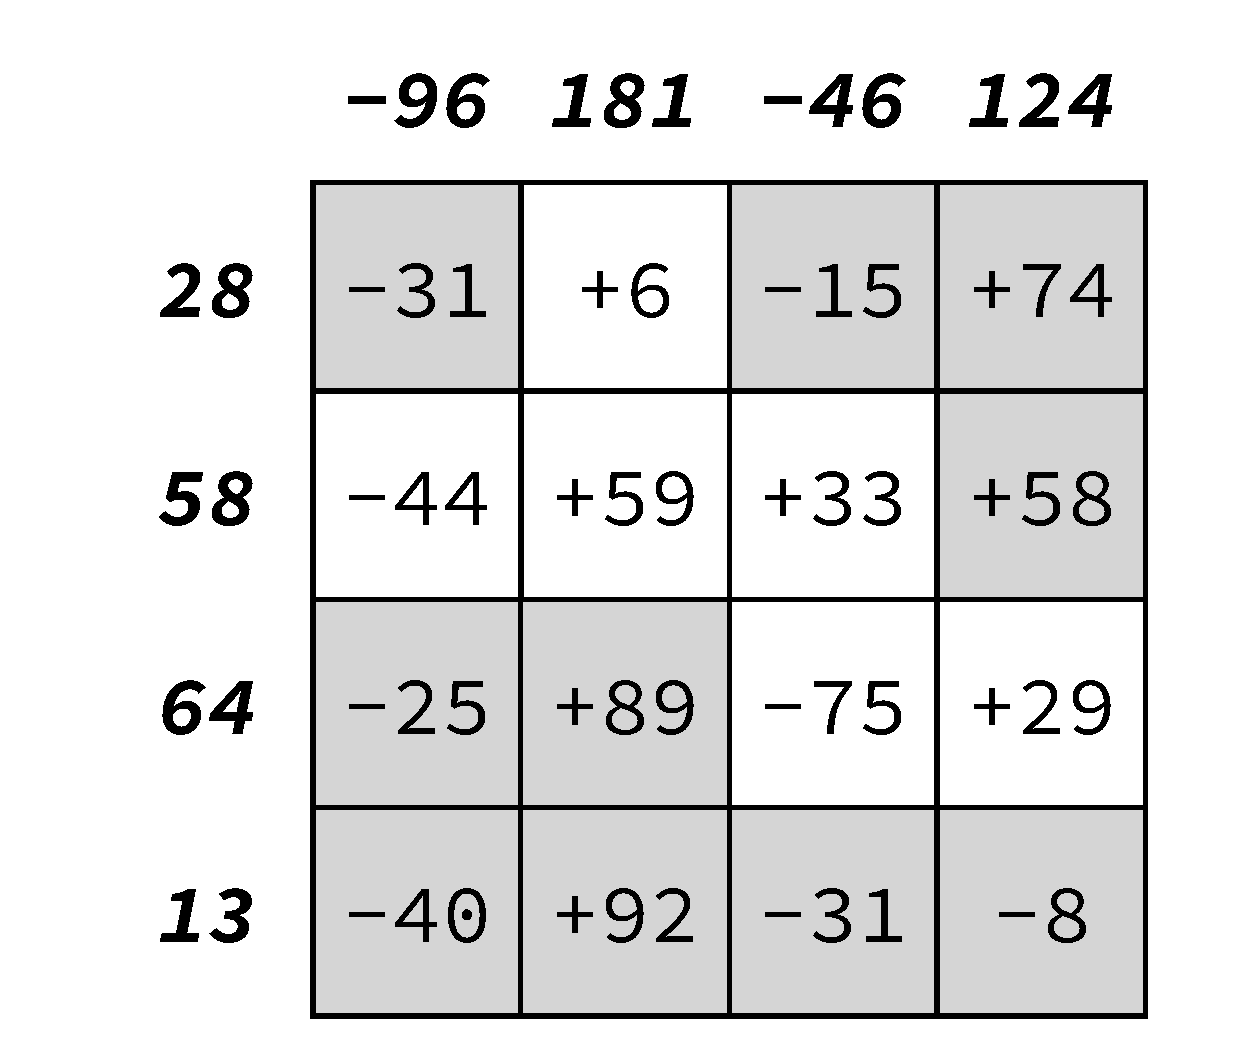
\includegraphics[scale=0.4,trim=0 30 0 30]{cswk/lac3s.pdf}
\end{center}
Finding a solution for a grid that cannot be solved in 0 moves is much harder than finding solutions for one that can be solved in 0 moves. In principle, we can use rotations to create an arbitrary arrangement of cells in the grid, thus leaving us with $(\mathit{rows} \times \mathit{columns})!$ many arrangements of cells. That means that for a $4 \times 4$ sized grid as the one shown above, there are $20,922,789,888,000$ many arrangements of cells. Each cell can then either be used or not, so for each of those arrangements there are $2^{4 \times 4}$ possible solutions, leaving us with a total state space of $(4 \times 4)! \times 2^{4 \times 4}$ many possible solutions. However, just finding a solution in itself does not tell us how to get there from the grid we start with, so a smarter approach is needed...

%-----------------------------------------------------------

\section{Getting started}
\label{sec:cswk1-getting-started}

In order to get started with the coursework, you need to get hold of the skeleton code and ensure that it compiles successfully on your machine. 

\subsection{Obtaining the skeleton code}

There are three different ways in which you can obtain the skeleton code for this coursework. All of them are explained below alongside their various advantages and disadvantages:

\paragraph{Option A: Private fork} By following the GitHub Classroom link below, you can create a private fork of our git repository with the skeleton code. This requires a GitHub account, but has the advantage that you have your own private copy of our repository on GitHub that you can write to. That would allow then you to work easily share your work between machines in the labs and at home:
\begin{center}
	\url{https://classroom.github.com/a/94xWYjXL}
\end{center}
Once you have accepted the assignment, you can then clone your fork of the skeleton code to your machine with the usual \bashIn{git clone} command where \texttt{\small [username]} is your GitHub username:
\begin{minted}{bash}
$ git clone https://github.com/fpclass/1920-cswk1-[username]
\end{minted}
\paragraph{Option B: Clone} If you do not wish to create a GitHub account or host a copy of your repository there, then you could instead just clone our repository with:
\begin{minted}{bash}
$ git clone https://github.com/fpclass/large-arithmetic-collider
\end{minted}
You will be able to \bashIn{git commit} changes to your local copy of the repository, but you will not be able to \bashIn{git push} them. This is sufficient if you are only planning to work on the coursework from one place (\emph{e.g.} only the lab machines but not your personal computer).

\paragraph{Option C: Archive} If GitHub should be unavailable or you do not have \bashIn{git} installed your machine, you can download a \texttt{\small .zip} file with the skeleton code from the module website.

\subsection{Working with the skeleton code}

You may wish to verify that the code compiles and that all tests fail by entering the \texttt{\small cswk1} directory that was created and running \bashIn{stack test}:
\begin{minted}{bash}
$ cd large-arithmetic-collider
$ stack test
\end{minted}
Running \bashIn{stack test} will compile your code, run a bunch of unit tests on it, and give you a rough indication of how complete your solution is (the more tests pass, the more complete it is). Running \bashIn{stack bench} will run a set of benchmarks on your code. You can also use \bashIn{stack build} to just compile your code and then \bashIn{stack exec mastermind} to run the program. Alternatively, you can run \bashIn{stack repl} to load up the REPL, which is useful for debugging.

The skeleton code contains a bunch of files, most of which you do not need to touch. The most important file is \texttt{\small src/Game.hs} which contains the definitions you will need to complete in order to implement the game. There are some definitions to get you started. Firstly, the arithmetic operations that may be contained in cells of the grids are represented as an algebraic data type where each constructor represent one type of operation:
\begin{minted}{haskell}
data Action 
  = Add Int 
  | Sub Int 
\end{minted}
Cells themselves are also represented as an algebraic data type comprised of a boolean value indicating whether the cell is enabled or not and an \haskellIn{Action} value representing the arithmetic operation contained in the cell:
\begin{minted}{haskell}
data Cell = Cell Bool Action
\end{minted}
Rows are comprised of a target number and a list of cells:
\begin{minted}{haskell}
data Row = Row Int [Cell]
\end{minted}
Finally, grids are comprised of a list of target numbers for all the columns and a list of all the rows in the grid:
\begin{minted}{haskell}
data Grid = Grid [Int] [Row]
\end{minted}

%-----------------------------------------------------------

%\section{Solving complex grids}



%-----------------------------------------------------------

\section{Task}

Complete all definitions in \texttt{\small src/Game.hs} so that the game works as described above. The following function stubs in \texttt{\small src/Game.hs}  need to be implemented:

\begin{enumerate}
	\item \haskellIn{eval :: Action -> Int -> Int}\\
	This function should apply an arithmetic operation represented by an \haskellIn{Action} value to an accumulator and return the result. For example, \haskellIn{eval (Add 5) 10} should evaluate to \haskellIn{15}.
	
	\item \haskellIn{result :: [Cell] -> Int}\\
	This function should determine the result of evaluating all the enabled arithmetic operations in a list of cells, starting with $0$. For example, evaluating \haskellIn{result [Cell True (Add 3), Cell False (Add 5)]} should result in \haskellIn{3}.
	
	\item \haskellIn{solveRow :: Row -> [Row]}\\
	This function should find all solutions for a given row.
	
	\item \haskellIn{solve :: Grid -> [Grid]}\\
	This function should find all solutions for a given grid, without rotating any rows or columns. If there are no solutions, an empty list should be returned.
	
	\item \haskellIn{rotations :: Grid -> [Grid]}\\
	Given a grid, this function should return a list of grids containing all possible ways to rotate the input grid. This means the resulting list should normally have $\mathit{rows} + \mathit{columns}$ many elements.
	
	\item \haskellIn{steps :: Grid -> [Grid]}\\
	If a grid cannot be solved without rotating it, this function should return a list of grids representing the shortest sequence of rotations which lead to a solution. I.e. the last grid in the list should be the solution and each grid should differ from the previous by exactly one rotation.
\end{enumerate}

%-----------------------------------------------------------

\section{Originality \& academic practice}

This coursework is an individual assignment and the work you submit must be entirely your own work. Students are expected to be familiar with the departmental Student Handbook as well as applicable university regulations. The ``Cheating and Plagiarism'' section on the handbook page about coursework is particularly relevant:
\begin{center}\small
	\url{https://warwick.ac.uk/fac/sci/dcs/teaching/handbook/coursework/}
\end{center}
Examples of what is not acceptable in the context of this assignment include, but are not limited to, the following:
\begin{itemize}
	\item Collaborating with others, for example by sharing code, looking at other people's code, or discussing implementation details such as which functions you used to implement a particular definition. 
	
	\item Copying or adapting code from web sources such as Stack Overflow, GitHub, etc. without attribution. This includes taking code written in other programming languages and translating it to Haskell. You may do this if you include a correct attribution to the source in e.g. a comment in your file, but note that you can only be awarded marks for work you have done yourself. 
\end{itemize}

%-----------------------------------------------------------

\section{Marking \& submission}

This coursework is worth 15\% of the overall module mark. It will be marked out of 100\% as follows:
\begin{itemize}
	\item 20\% for \emph{correctness and documented understanding (basic grids)}. You gain full marks here if all parts of the coursework required to solve basic grids (up to and including the \haskellIn{solve} function) been attempted and are correct. You may use \bashIn{stack test} as a rough indication for whether this is the case, but there are some things the unit tests do not test for, so you should play the game and ensure that everything works as described. You should also document your code with comments and explain how it works. You gain full marks if all code is documented and explained sufficiently well so that someone who is unfamiliar with your code can understand it.
	
	\item 20\% for \emph{correctness and documented understanding (advanced grids)}. You gain full marks here if all parts of the coursework required to solve advanced grids (the \haskellIn{steps} function) been attempted and are correct. You may use \texttt{\small stack test} as a rough indication for whether this is the case, but there are some things the unit tests do not test for, so you should play the game and ensure that everything works as described. You should also document your code with comments and explain how it works. You gain full marks if all code is documented and explained sufficiently well so that someone who is unfamiliar with your code can understand it.
	
	\item 20\% for \emph{elegance}. Definitions should be concise and readable, new functions should be introduced where needed, existing library functions used when applicable, etc.
	 
	\item 20\% for \emph{performance and efficiency}. You will do well here if you use sensible data structures and your functions perform as little redundant computation as possible. You can test performance by running \texttt{\small stack bench} on different versions of your code to see how they compare. 
	
	\item 20\% for \emph{improvements and extensions}. This is an opportunity for you to demonstrate creativity and advanced understanding. You could achieve this in many different ways, such as adding additional unit tests, functionality, improved algorithms, etc. You may wish to modify \texttt{\small app/Main.hs} as well as other source files or even add new ones. You could also prove some properties about your game on paper. The amount of marks awarded will depend on the complexity and creativity of your extension(s) and improvement(s).
\end{itemize}
Submit a \texttt{\small .zip} or \texttt{\small .tar.gz} archive of the whole, completed project (not just \texttt{\small Game.hs}) through Tabula by \deadlineOneTime\ on \deadlineOneDate:
\begin{center} 
	\url{\submissionOneURL}
\end{center}
